We executed the approach mentioned in the \textbf{Section - 4} on both \textit{Linear Regression} and \textit{XGBoost} algorithms.
As shown in the Fig - \ref{fig:bio_age_results_comp_with_test_data} Linear Regression performs worse and is concentrated around somewhere between 75-85 for most test samples. However, XGBoost shows Gaussian distribution and scattered nicely, which shows better fit.

\begin{figure}[H]
	\def\imgwidth{0.5\linewidth}
	\centering
	\begin{tabular}{cc}
		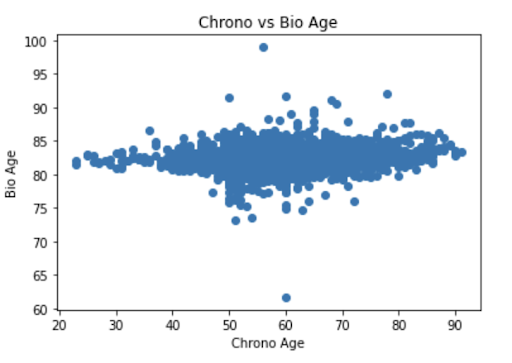
\includegraphics[width=0.4\linewidth]{images/bio_age/bio_lr.png} &
		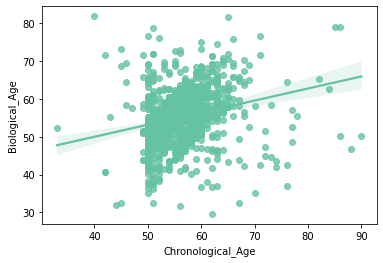
\includegraphics[width=0.4\linewidth]{images/bio_age/bio_xgboost.png} \\
	\end{tabular}
	\caption{Biological Age: comparison of both the algorithm on test-data left=Linear Regression, right=XGBoost}
	\label{fig:bio_age_results_comp_with_test_data}
\end{figure}

Next, we show in Fig - \ref{fig:bio_age_results_body}  correlation of features such as muscle mass, muscle area and calcification with Biological age. Muscle Mass and Muscle Area are decreasing as Biological age increases. Calcification is increasing as Biological age increases.

\begin{figure}[H]
	\def\imgwidth{0.5\linewidth}
% 	\setlength\tabcolsep{2pt}
	\centering
	\begin{tabular}{ccc}
		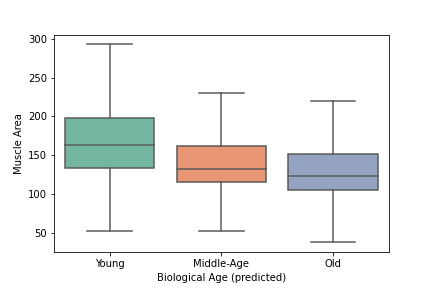
\includegraphics[width=0.3\linewidth]{images/bio_age/bio_muscle_area.png} &
		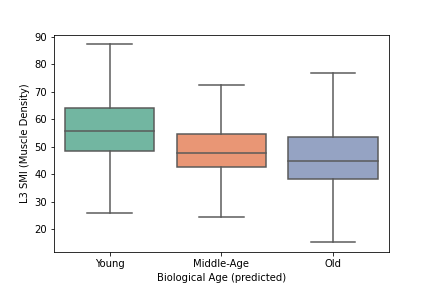
\includegraphics[width=0.3\linewidth]{images/bio_age/bio_muscle_mass.png} &
		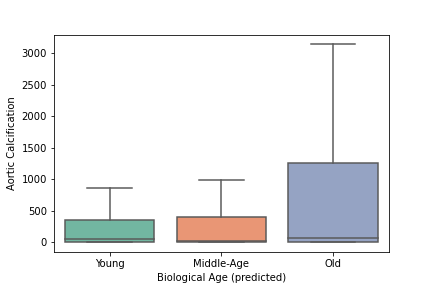
\includegraphics[width=0.3\linewidth]{images/bio_age/bio_calci.png} \\
	\end{tabular}
	\caption{Effect on body as bio age is increasing. left = decreasing muscle area, center = decreasing muscle mass, right = increasing calcification}
	\label{fig:bio_age_results_body}
\end{figure}